\chapter{Asking Salt Lake City Millionaires How They Got Rich}

This chapter comes from an interview lecture rather than a blackboard lecture, but it still unfolds with a definite quantitative rhythm. We begin with a montage of wealth claims, pass into execution under a new technological regime, then move through a real-estate compounding mechanism, owner-level accounting, arbitrage, concentration of effort, and finally the cash discipline that the speakers treat as the precondition of independence. The governing rule for these notes is simple: we formalize only what the transcript genuinely supports, and we keep the order of motivation close to the way the lecture itself advances.

\section{Opening Stakes and the Promise of Rebuildable Wealth}

The lecture begins by dazzling us. We see expensive signals, hear about eight-figure annual income, many companies, and the claim that one could start over at a job paying \$3{,}000 a month and, within a year, become a millionaire again. This opening is not yet an argument. It is a wager with the audience: wealth here will be presented not merely as visible scale, but as something that can, at least in principle, be rebuilt.

Only after that wager is placed does the host state the governing premise. We are going around the wealthier parts of Salt Lake City to ask successful business owners how they became wealthy and what someone else might do now to begin a path toward financial freedom. The lecture therefore proceeds case by case. It does not begin with a single theorem; it begins with a promise that concrete mechanisms will be extracted from concrete operators.

\section{Execution Before Glamour}

The first entrepreneur is introduced through scarcity and scale at once. We are told that he came to Utah with \$50, later did over \$600 million in roughly a decade, and attributes the transformation to one word repeated like a drumbeat: execution. In the lecture this is not empty emphasis. It is the baseline explanatory principle to which the interview repeatedly returns.

The first named financial decision is the building of the biggest Bitcoin mining facility in Utah in 2014. What matters is not only the sector, but the posture. The speaker describes the move as partially accidental: the firm was already a computer company, already had the hardware, and simply connected the video cards and began mining. That anecdote then widens into a more general thesis. Blockchain and AI are presented as contemporary versions of the early internet, still strange enough that many dismiss them, but structured enough that an early entrant can build against the next layer of demand.

The transcript then compresses a further claim about the future of the economy. Government digital currency, tokenization of real-world assets, and the early movement of large institutions such as BlackRock are mentioned as signs that the rails themselves are changing. The chronology of crypto involvement is slightly compressed in the transcript, so we should not over-specify the timeline. What the lecture clearly wants us to keep is the structure of the opportunity: execution matters most when it is joined to a frontier that is still being misread by the majority.

\subsection{Question \& Answer}

The lecture now tests its own optimism. What is the lowest point, and how does one return from it?

The answer is severe enough to change the tone of the chapter. A bad marketing manager loses \$800{,}000 in 90 days. Seventy-five people are laid off. This matters because it breaks the glamour of the teaser montage and forces the lecture to specify what, if anything, survives after a major operational failure.

The recovery logic is given in plain speech, but it has a clear order:

\begin{enumerate}
\item stop the immediate damage;
\item shrink the organization to match reality;
\item return to the books;
\item bring in strong tax and accounting help;
\item talk to mentors;
\item frame the problem clearly;
\item execute again.
\end{enumerate}

The lecture claims that recovery came within 12 months. We are not given the full cash-flow path and should not invent one. But we are given a recoverability model: not confidence in the abstract, but disciplined reduction back to the variables one can still control.

That is why the next question lands cleanly. If everything were lost tomorrow, could it all be made back? The answer is yes. The compressed reason is selling. This serves as the bridge back from adversity to repeatability. The entrepreneur then says that entering tech in 2024 should be understood the way the internet could have been understood in the early 1990s: as a period when the infrastructure is still new, the problems are still forming, and the great asymmetry belongs to those who arrive before the crowd fully believes.

\section{Real Estate as a Recursive Compounding Machine}

The host then resets the lecture's energy and moves us to a different terrain. We leave the first entrepreneur's frontier-tech case and arrive at Chris Krohn's estate. The problem changes with the setting. We are no longer being asked how to enter a new technological wave; we are now being asked how capital itself can be made to propagate.

Chris Krohn states his origin in strongly numerical terms. He started in real estate, began with a small portfolio of 25 homes, says that this was enough to avoid needing a job after college, and later describes the portfolio as having grown into thousands of homes. He also states that he has cleared over \$10 million in a year. This is precisely the moment when the lecture pivots from scale to mechanism.

\subsection{Question \& Answer}

The host now asks the first properly constructive question of this segment: if one does not already have a great deal of money, what first actionable move can one take in real estate?

The answer is house hacking. The lecture gives just enough arithmetic to formalize the skeleton without pretending to supply a full underwriting model.

\begin{definition}
For house \(n\), let \(P_n\) denote the purchase price, \(V_n\) the market value, \(L_n\) the loan balance, \(D_n\) the down payment, and \(E_n\) the equity.
\end{definition}

The first step is stated directly:
\begin{align}
D_1 &= 0.03\,P_1,\\
P_1 &< V_1,\\
E_n &= V_n - L_n.
\end{align}

The verbal structure is then straightforward. Buy the first house with a \(3\%\) down payment. Buy below market. The gap between market value and debt creates equity. Strip some usable portion of that equity out and let it seed the next acquisition. In schematic form,
\begin{equation}
E_1 \to D_2,\qquad E_2 \to D_3.
\end{equation}

\paragraph{Worked chain.}
The recursive logic can be written in a deliberately cautious sequence:

\begin{enumerate}
\item Acquire the first property with a low initial cash commitment:
\[
D_1 = 0.03\,P_1.
\]
\item Buy below market so that acquisition does not merely consume cash but creates embedded equity:
\[
P_1 < V_1.
\]
\item Write the resulting equity as
\[
E_1 = V_1 - L_1.
\]
\item Refinance or otherwise extract part of \(E_1\), and use that extracted capital as the next seed \(D_2\).
\item Repeat the logic at the next step. The second house helps finance the third, and the portfolio begins to grow recursively rather than linearly.
\end{enumerate}

The lecture does not tell us the refinance ratio, the appraisal timing, the interest structure, or the holding period. It tells us something more elementary and, within the lecture, more important: wealth in real estate begins when capital stops being static and begins to move.

\begin{figure}
\centering
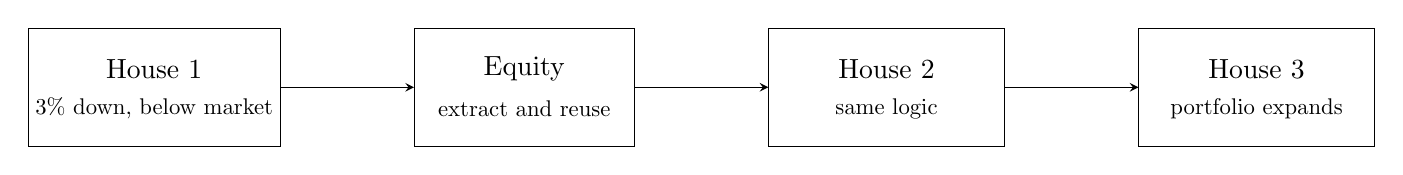
\begin{tikzpicture}[x=1cm,y=1cm,>=stealth]
\draw (0,0) rectangle (3.2,1.5);
\node at (1.6,0.98) {House 1};
\node[scale=0.82] at (1.6,0.48) {$3\%$ down, below market};

\draw[->] (3.2,0.75) -- (4.9,0.75);

\draw (4.9,0) rectangle (7.7,1.5);
\node at (6.3,0.98) {Equity};
\node[scale=0.82] at (6.3,0.48) {extract and reuse};

\draw[->] (7.7,0.75) -- (9.4,0.75);

\draw (9.4,0) rectangle (12.4,1.5);
\node at (10.9,0.98) {House 2};
\node[scale=0.82] at (10.9,0.48) {same logic};

\draw[->] (12.4,0.75) -- (14.1,0.75);

\draw (14.1,0) rectangle (17.1,1.5);
\node at (15.6,0.98) {House 3};
\node[scale=0.82] at (15.6,0.48) {portfolio expands};
\end{tikzpicture}
\caption{Transcript-derived sketch of the house-hacking capital ladder. The lecture gives the mechanism verbally: one property seeds the next through embedded equity.}
\end{figure}

The transcript slightly garbles the final wording of this answer, but the intended meaning is still clear: high-volume real-estate activity is not imagined here as waiting passively for large initial wealth. It is imagined as learning how to make capital reproduce itself.

\section{The Language of Business and the Spread of Arbitrage}

The interview does not remain inside real estate for long. Once the acquisition ladder is on the table, the host asks a different question: what prevents owners from scaling and lasting? The answer is as sharp as it is simple. They trust their accountants. They trust their CFOs. The speaker's point is not that accountants are unnecessary. It is that the owner must remain able to read the business directly.

\begin{definition}
Let \(R\) denote gross revenue, \(X\) expenses, \(\Pi\) retained profit, and \(m\) margin.
\end{definition}

The minimal accounting identities are then
\begin{align}
\Pi &= R - X,\\
m &= \frac{\Pi}{R}.
\end{align}

The lecture's emphasis here is operational rather than scholastic. One may generate large revenue and still keep very little of it. If the owner does not understand margin, gross revenue, and expenses firsthand, then the business may look impressive from the outside while remaining hollow in retained value. That is what is meant when the speaker says that the language of business is accounting.

\subsection{Question \& Answer}

The next question is explicit: what lesson about money would somebody fail to learn in business school?

The answer is financial arbitrage. The lecture presents it in a stripped-down form that invites formalization. Borrow money at a low rate; deploy it at a higher rate; capture the difference.

Write
\begin{align}
\Delta r &= r_{\text{earn}} - r_{\text{borrow}},\\
W_{\text{spread}} &= K\,\Delta r = K\bigl(r_{\text{earn}} - r_{\text{borrow}}\bigr),
\end{align}
where \(K\) is deployed capital, \(r_{\text{borrow}}\) is the borrowing rate, and \(r_{\text{earn}}\) is the earning rate on the investment.

The transcript gives example values rather than a complete finance model:
\[
r_{\text{borrow}} \in \{3\%,5\%,7\%\},\qquad
r_{\text{earn}} \in \{25\%,50\%,100\%\}.
\]

\paragraph{Worked example.}
If we take
\[
r_{\text{borrow}} = 5\%,\qquad r_{\text{earn}} = 25\%,
\]
then
\[
\Delta r = 25\% - 5\% = 20\%,
\]
and hence
\[
W_{\text{spread}} = 0.20\,K.
\]

This is exactly the quantity the speaker calls ``the middle part.'' In the lecture, that middle part is not merely a financial spread. It is the reward for understanding the game well enough not to surrender control of capital to someone else. The formula therefore captures both the arithmetic and the lecture's moral emphasis. We should still be cautious: no taxes, leverage limits, risk adjustments, or time conventions are supplied, so the equation remains a clean heuristic rather than a full pricing model.

From here the lecture widens again. The host asks what keeps people broke. Chris Krohn answers not first with interest rates or balance sheets, but with social friction: poor people take advice from poor people; crab-bucket dynamics pull ambitious actors downward; and fear of losing family and friends keeps many from making financially different choices. This is a transition of real importance. After arbitrage, the lecture reminds us that even a correct model of wealth is not enough if the surrounding social field punishes deviation from the familiar.

\section{Lifestyle Compression and Concentrated Bets}

The host then resets the lecture once more and brings us to Keaton Hoskins. The rhythm changes again. This segment opens not with a specific asset class, but with entrepreneurship as total identity. Hoskins says he has built 35 companies since age 21 and, when asked what industry he chose, answers in effect: any industry in which a business could be started.

The first substantive rule, however, is not about unlimited expansion. It is about compression. One should learn how to downgrade lifestyle so that one can later upgrade life. The lecture ties this to a quoted statistic: one in four millionaires still live paycheck to paycheck because they refuse to compress consumption even temporarily. Whether or not we verify that statistic elsewhere, its role in the lecture is clear. Wealth is being separated from visible spending.

The next move is even tighter. Money should be dumped into only two things: the self and the business. The more one invests in oneself, the more one makes; the more one invests in the business, the more the business makes. The point is not generic thrift. The point is that reinvestment must be concentrated in channels with compounding force.

\subsection{Question \& Answer}

At exactly this point the host raises the next natural tension. Many people make some money and immediately want to diversify across industries. How important is it, instead, to become world-class at one thing or at most a few things?

The answer is intentionally blunt: go deep. The lecture opposes a shotgun allocation of effort to a concentrated allocation of effort. We can state that logic with a simple normalization.

Let \(a_i\) be the share of total available effort, attention, or capital allocated to project \(i\). Then
\begin{equation}
\sum_{i=1}^{N} a_i = 1.
\end{equation}

If one spreads oneself over five directions at once, the lecture's implicit model is
\begin{equation}
a_i = 0.2\qquad (i=1,\dots,5).
\end{equation}
If one commits fully to a single direction, then
\begin{equation}
a_1 = 1.
\end{equation}

The speaker's claim is that significance belongs to the second pattern rather than the first. This is not a theorem of optimal portfolio selection. It is a model of depth. Spread scarce attention too widely and no single undertaking gets enough density to break through. Concentrate it and one thing can be crushed.

\begin{remark}
The lecture's argument here is motivational and strategic, not formal portfolio theory. We preserve it as a model of depth versus dilution.
\end{remark}

The transcript immediately gives us a concrete version of the same point. Someone arrives with \$100{,}000 and wants simultaneously to do the stock market, Bitcoin, start a business, buy a business, and several other things besides. The lecture's answer is no. Find one thing you can get behind. In the logic of the chapter, this is the same doctrine we have already seen twice under different names: first as execution, then as capital recycling, and now as concentrated allocation.

\section{Question \& Answer: What Does It Mean To Be Broke?}

The final turn of the lecture is psychologically sharper than the earlier ones. The host asks whether Hoskins has ever been broke. The answer is surprising: honestly, no. The speaker then explains that there were moments when he had only \$100 in his bank account, including when his father died, but he does not define ``broke'' as merely having a small balance. He defines it as needing rescue.

That redefinition leads to the lecture's starkest heuristic:
\begin{equation}
\neg \mathrm{Manage}(100)\Rightarrow \neg \mathrm{Manage}(10^5),\qquad
\neg \mathrm{Manage}(100)\Rightarrow \neg \mathrm{Manage}(10^6).
\end{equation}

This is not a theorem and should not be dressed up as one. It is a scaling claim about behavior. If one cannot manage small sums, then larger sums will not repair the underlying pattern.

The lecture then turns this principle into a rough austerity sketch. Suppose monthly income is
\begin{equation}
I = 3000.
\end{equation}
Let \(H_{\text{share}}\) be personal housing cost, \(T\) transport, \(M\) meals, and \(Q\) all remaining outlays. Then a minimal monthly surplus can be represented by
\begin{equation}
S = I - \bigl(H_{\text{share}} + T + M + Q\bigr).
\end{equation}
The transcript also gives a specific housing anchor:
\begin{equation}
H = 1000,
\end{equation}
with the housing cost then split among multiple occupants, so that
\begin{equation}
H_{\text{share}} = \frac{H}{N}.
\end{equation}

The transcript leaves \(N\) somewhat ambiguous, because ``find four roommates'' does not pin down the total number of people in the unit with complete precision. But that ambiguity does not affect the lecture's point. The point is that \(Q\), the category of nonessential outflow, must be driven aggressively toward zero if capital is to accumulate.

From here the lecture states its final doctrine without apology. People stay broke because they spend too much on things they do not need and because they believe they are owed a certain lifestyle. A certain house, a certain car, a certain watch, a certain visible level of comfort: all of this is treated as pre-claimed consumption. In the arithmetic of the chapter, entitlement is simply a name for rigid discretionary spending.

We can therefore summarize the final mechanism in four short lines:
\begin{itemize}
\item small balances are not the deepest problem;
\item unmanaged spending is;
\item status consumption competes directly with reinvestment;
\item temporary austerity is presented as the price of independence.
\end{itemize}

The final cultural examples are rhetorically strong and should be handled with care in interpretation. Still, the logical structure is plain. Wealth here is not defined by what one can display; it is defined by whether one can retain surplus, redeploy it, and avoid being owned by fixed expectations of comfort.

\section{Summary}

The lecture begins with visible scale and then spends the rest of its time trying to explain why visible scale is not the true engine. The deeper engine is execution on a frontier, recovery after failure, recursive capital motion in real estate, owner-level fluency in accounting, spread capture through arbitrage, concentrated deployment of effort, and discipline severe enough to resist entitlement. The mathematics is therefore modest but real: equity is created and recycled, profit is distinguished from revenue, spreads are computed, attention is allocated, and surplus appears only when fixed claims on lifestyle are compressed. That is the commercial arithmetic by which this lecture says wealth is made, lost, and made again.